\section{Design}

\subsection{Nodes}

\subsubsection{Components}

The first step in the design process was selecting hardware components that
could operate autonomously without mains power. This required devices that were
highly power-efficient, while also capable of transmitting small data
packets via LoRa. An equally important consideration was ensuring the final
devices could be fully weatherproofed to protect the sensitive electronics from
water ingress and environmental damage.

\paragraph{Challenger RP2040 LoRa}

The iLabs Challenger RP2040 LoRa is an embedded computer that uses the Raspberry Pi
RP2040 chip that was released in 2021. The RP2040 itself is a low-cost and
power-efficient processor with ample power to perform the data encoding and
transmission in my use case. Additionally, the chip is extremely popular with
over 10 million units being produced in the first two years of release
\cite{pounder2023}. This popularity means there is ample documentation for
developing with this processor and is compatible with circuit python which was
my preferred language for development on the nodes.

\begin{figure}[H]
    \centering
    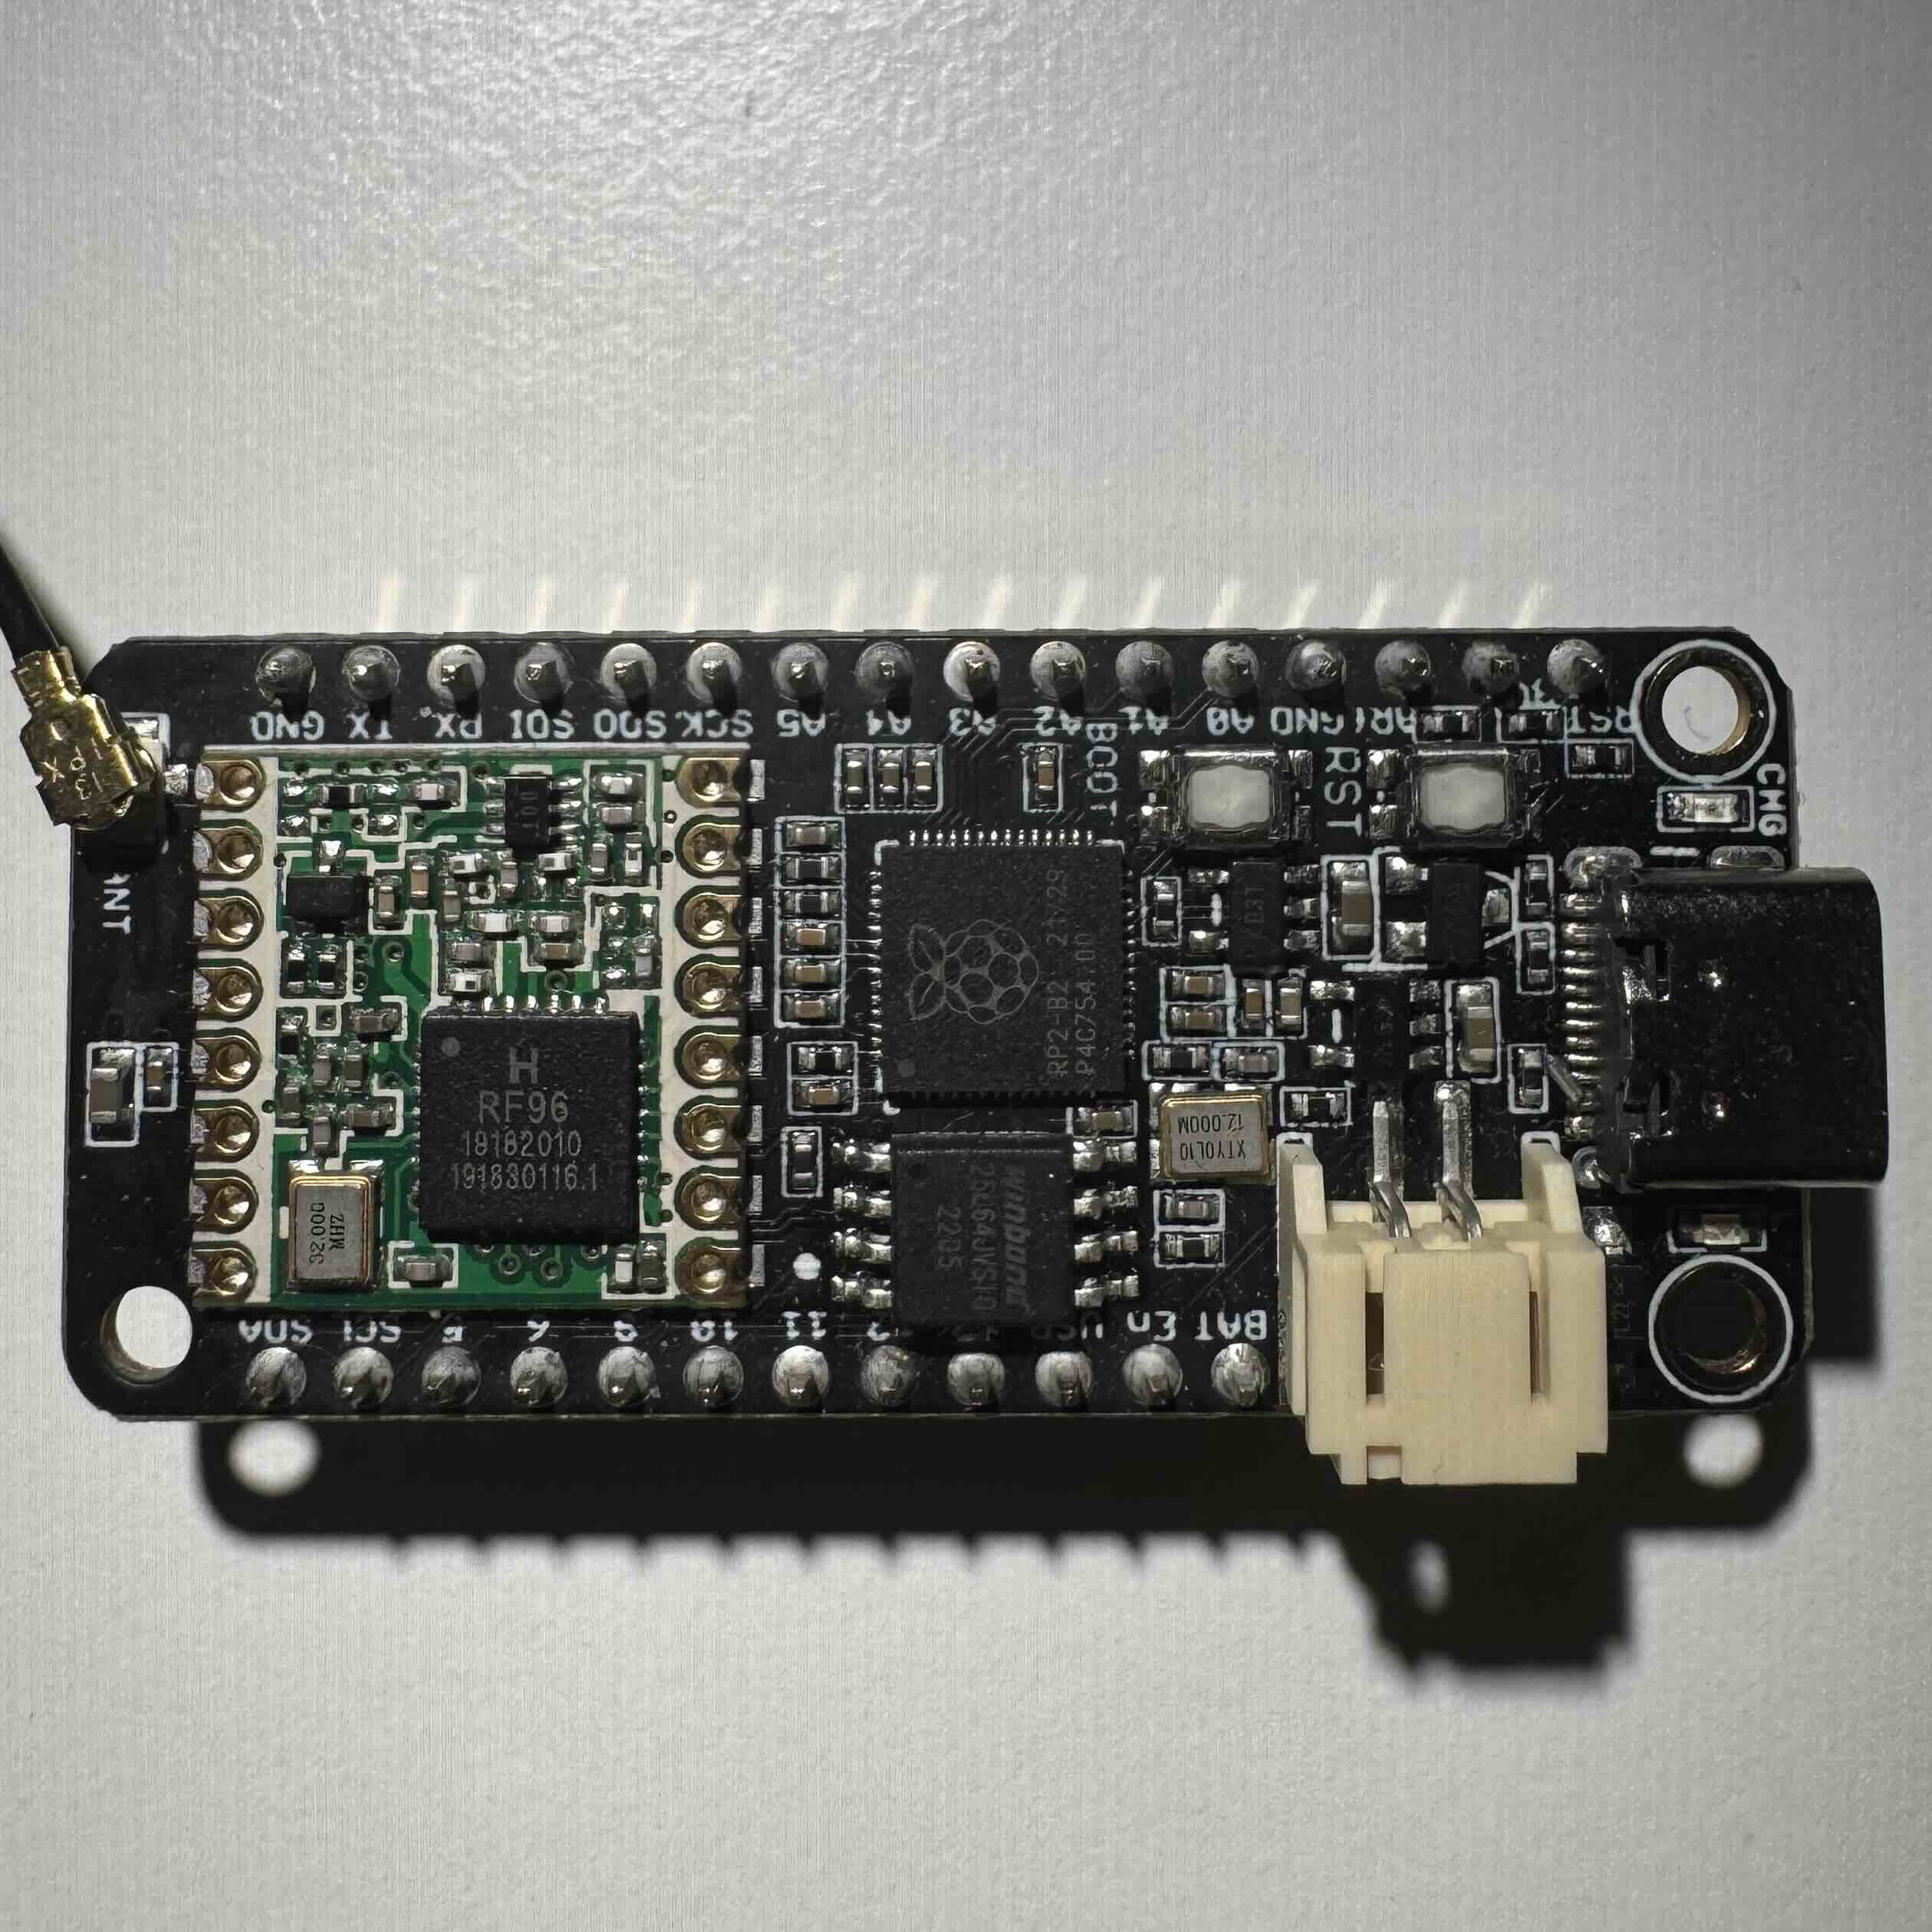
\includegraphics[width=0.5\textwidth]{contents/22-hw-design/22-fig/challenger-rp2040.jpg}
    \caption{iLabs Challenger RP2040 used in the project. Note the RP2040 chip centre and RF96 LoRa module to the left.}
\end{figure}

The challenger board itself is based on the Adafruit feather form factor

\paragraph{Antennae}

\paragraph{Sensor selection}

\subparagraph{Temperature and humidity sensor}

\subparagraph{Soil moisture sensor}

\subparagraph{Wind speed sensor}

\paragraph{Powering the node}

\paragraph{Weather proofing}

\subsubsection{Repeater}

\subsection{Gateway}

\subsection{LoRa settings}

\subsubsection{Compliance with regulatory limits on radio power}